\chapter{Introduction}

\section{Context and Motivation}

\subsection{Evolution of Software Deployment Methodologies}
The landscape of software deployment has undergone significant transformation in recent years, driven by the increasing complexity of modern applications and the demand for faster, more reliable delivery cycles. Traditional deployment approaches, characterized by manual processes and sequential workflows, have evolved into sophisticated automated methodologies that emphasize continuous integration and deployment practices.

Modern enterprise environments increasingly rely on complex distributed architectures comprising multiple microservices, each with distinct technology stacks, deployment requirements, and operational characteristics. These architectures span multiple cloud providers, leverage \textbf{\hyperref[docker2023documentation]{containerization technologies}}, and require \textbf{\hyperref[kubernetes_docs]{advanced orchestration mechanisms}} to ensure reliable operation across diverse environments.

\textbf{\hyperref[fowler2013continuous]{Traditional Continuous Integration and Continuous Deployment (CI/CD) methodologies}} have successfully automated many aspects of the software delivery pipeline, including build processes, testing procedures, and deployment orchestration. However, these approaches face mounting challenges in contemporary enterprise environments, particularly regarding manual approval gates, multi-environment consistency management, and complex rollback procedures that require human intervention.

\subsection{GitOps Emergence and Industry Interest}
GitOps represents a paradigmatic shift toward declarative deployment methodologies that leverage Git repositories as the single source of truth for both application code and infrastructure configuration. This approach fundamentally transforms the deployment model from imperative command execution to desired state convergence, where automated controllers continuously monitor Git repositories and ensure that deployed environments match declared specifications.

The declarative nature of GitOps enables enhanced automation capabilities including automatic drift detection, self-healing mechanisms, and simplified rollback procedures through Git revision management. GitOps controllers such as \textbf{\hyperref[argo_cd_docs]{ArgoCD}} and \textbf{\hyperref[flux2023]{Flux}} provide advanced monitoring and synchronization capabilities that can automatically detect and correct configuration drift without human intervention, promising improved operational reliability and enhanced audit capabilities.

Despite growing industry interest and academic attention, fundamental questions about GitOps practical performance characteristics remain inadequately addressed. Current literature predominantly focuses on theoretical advantages without providing comprehensive empirical validation against established Traditional CI/CD methodologies, creating uncertainty around adoption strategies and implementation decisions for enterprise organizations.

\subsection{Research Motivation and Critical Gaps}
The motivation for this research stems from the critical gap between theoretical GitOps promises and practical implementation realities in enterprise software development environments. While academic literature extensively discusses conceptual advantages such as declarative state management, enhanced security through Git-based audit trails, and simplified multi-environment orchestration, empirical validation using production systems remains severely limited.

Enterprise decision-makers require quantitative evidence to assess the trade-offs between deployment speed, operational automation, failure recovery capabilities, and resource utilization across different methodological approaches. Without empirical data from production systems, organizations must base critical technology decisions on vendor claims, theoretical analyses, and limited case studies that may not reflect their specific operational context and requirements.

The absence of rigorous comparative studies using production-grade environments creates uncertainty around GitOps adoption strategies, hybrid implementation approaches, and optimization opportunities. Organizations need evidence-based frameworks to evaluate methodology selection, migration strategies, and performance optimization, yet current research provides insufficient guidance for these critical decisions.

\section{Problem Statement and Research Challenges}

\subsection{Lack of Empirical Evidence in Methodology Comparison}
Current GitOps research predominantly focuses on conceptual frameworks and theoretical benefits without providing comprehensive empirical validation against Traditional CI/CD methodologies. Academic studies typically examine GitOps principles in isolation or through limited demonstration scenarios that fail to capture the complexity and operational constraints of real-world enterprise environments.

The absence of standardized comparison methodologies compounds this challenge, as existing studies often employ different metrics, environments, and evaluation criteria that prevent meaningful cross-study analysis. This fragmentation makes it difficult for organizations to synthesize available research into actionable decision frameworks for methodology selection and implementation planning.

Enterprise practitioners consistently express uncertainty about GitOps adoption decisions due to the lack of comprehensive performance data that accounts for real-world operational constraints, service complexity variations, and technology stack diversity. This uncertainty is particularly pronounced in organizations with significant investments in existing Traditional CI/CD infrastructure.

\subsection{Service Complexity and Technology Stack Variations}
Modern enterprise applications comprise diverse microservices implemented using different programming languages, frameworks, and technology stacks. Each service exhibits distinct complexity characteristics including codebase size, dependency relationships, resource requirements, and operational patterns that significantly impact deployment performance and operational behavior.

Traditional performance evaluations often compare methodologies using homogeneous test environments that do not reflect the heterogeneous nature of real-world application portfolios. This limitation prevents accurate assessment of methodology performance across different service types and complexity levels, potentially leading to biased conclusions that favor specific technology stacks rather than methodological approaches.

The challenge becomes particularly acute when evaluating hybrid architectures where different services may benefit from different deployment methodologies based on their complexity, criticality, and operational requirements. Organizations need frameworks that can account for service-specific characteristics while providing fair methodology comparisons.

\subsection{Production Environment Validation Requirements}
Laboratory testing environments and synthetic benchmarks, while useful for controlled experimentation, often fail to capture the operational complexity and resource constraints characteristic of production systems. Real-world deployments involve network latency, resource contention, security scanning, compliance checking, and integration dependencies that significantly impact performance characteristics.

Production environments introduce variability factors including dynamic resource allocation, concurrent user loads, database performance fluctuations, and external service dependencies that cannot be replicated in simplified test environments. These factors are critical for accurate methodology evaluation as they directly impact deployment success rates, performance consistency, and recovery characteristics.

\subsection{Integration and Migration Strategy Challenges}
Organizations face practical challenges when considering GitOps adoption, particularly regarding integration with existing Traditional CI/CD infrastructure and migration strategies for complex application portfolios. The assumption that methodologies are mutually exclusive creates unnecessary constraints that may prevent gradual adoption approaches and hybrid architecture implementations.

Current research provides limited guidance on methodology coexistence, cross-methodology integration patterns, and performance implications of hybrid deployments. Organizations need evidence-based frameworks to evaluate whether methodologies can complement each other, what integration overhead might be expected, and how migration strategies can be optimized.

\section{Research Objectives and Questions}

\subsection{Primary Research Objectives}
The primary objective of this research is to conduct the first comprehensive empirical comparison of GitOps and Traditional CI/CD methodologies using a production-grade multi-service platform with complexity normalization and statistical validation. This investigation aims to provide evidence-based insights for enterprise methodology selection decisions while identifying concrete optimization opportunities for both approaches.

The research addresses the critical gap between theoretical GitOps concepts and practical implementation realities by developing and analyzing a functional production system that serves as both a research platform and a demonstration of methodological capabilities. This approach ensures findings reflect genuine deployment characteristics rather than laboratory conditions or theoretical projections.

\subsection{Specific Research Questions}
This study addresses five fundamental research questions that bridge the gap between theoretical concepts and practical implementation realities:

\textbf{Research Question 1:} How do GitOps and Traditional CI/CD methodologies compare in deployment performance when normalized for service complexity and technology stack variations?

\textbf{Research Question 2:} Can GitOps and Traditional CI/CD methodologies coexist effectively in hybrid architectures without introducing significant performance penalties or operational complexity?

\textbf{Research Question 3:} What are the quantifiable trade-offs between build speed and operational automation across different methodology approaches?

\textbf{Research Question 4:} What are the primary performance bottlenecks and optimization opportunities for each methodology in production environments?

\textbf{Research Question 5:} Which methodology approach is optimal for different organizational contexts including team size, operational requirements, and performance priorities?

\subsection{Research Scope and Boundaries}
The implementation scope encompasses four production microservices deployed across multiple cloud providers using both GitOps and Traditional CI/CD methodologies, with comprehensive monitoring infrastructure for performance measurement and statistical validation. The study deliberately focuses on production system validation using real workloads and operational constraints.

The research boundaries include evaluation of deployment performance, operational automation, failure recovery capabilities, and cross-methodology integration patterns. The study excludes detailed security analysis, compliance frameworks, and long-term operational cost analysis, focusing instead on performance characteristics and operational effectiveness.

\section{Methodology and Research Approach}

\subsection{TechMart Platform Implementation}
To address the empirical validation requirements, this study implements TechMart, a comprehensive production-grade e-commerce platform designed specifically for rigorous methodology comparison. TechMart serves dual purposes as both a functional multi-cloud application demonstrating realistic business capabilities and a controlled research environment enabling systematic performance measurement.

The platform architecture encompasses four distinct microservices: User Service (Python FastAPI + PostgreSQL), Order Service (Python FastAPI + PostgreSQL + Redis), Product Service (Node.js Express + MongoDB), and Cart Service (Java Spring Boot + Redis). This technology diversity enables evaluation of methodology performance across various programming languages and frameworks while maintaining architectural coherence.

TechMart operates as a live production system accessible at the ecommerce-microservices-platform repository, implementing authentic multi-cloud deployment patterns spanning Google Cloud Platform, Heroku, Vercel, and Azure infrastructure to create realistic operational complexity for methodology evaluation.

\subsection{Two-Phase Research Design}
The research employs a systematic two-phase approach designed to establish baseline characteristics before conducting comprehensive comparative analysis. Phase 1 focuses on single-service controlled comparison to establish fundamental performance characteristics and identify key variables affecting methodology performance.

Phase 2 implements multi-service complexity normalization to enable fair cross-methodology evaluation while accounting for service heterogeneity and technology stack variations. This progressive approach ensures both methodological rigor and practical relevance for enterprise decision-making.

Figure \ref{fig:research_methodology} illustrates the systematic two-phase research methodology framework that guides this empirical investigation, showing the progression from controlled baseline analysis to comprehensive multi-service complexity normalization.

\begin{figure}[H]
\centering
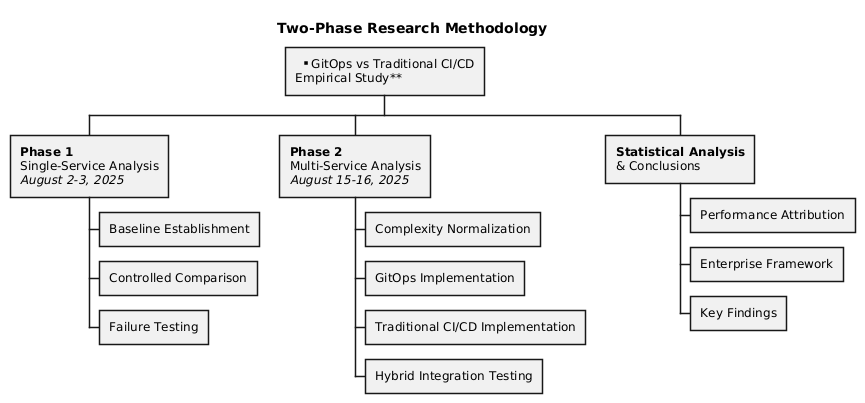
\includegraphics[width=\textwidth]{figures/research-methodology.png}
\caption{Two-Phase Research Methodology for GitOps vs. Traditional CI/CD evaluation.}
\label{fig:research_methodology}
\end{figure}

\subsection{Complexity Normalization Framework}
The study develops a novel complexity normalization framework that enables fair comparison across heterogeneous service architectures by accounting for codebase complexity, build requirements, resource intensity, technology stack characteristics, external dependencies, and deployment target complexity. This framework addresses fundamental challenges in DevOps research where service complexity variations can obscure methodology-specific performance characteristics.

\section{Expected Contributions and Impact}

\subsection{Technical and Academic Contributions}
The study's technical contributions include the development of the complexity normalization framework that enables fair comparison across heterogeneous service architectures, eliminating technology stack bias from methodology evaluation. This framework addresses a fundamental challenge in DevOps research and establishes new standards for CI/CD methodology comparison.

The research provides the first empirical validation of hybrid GitOps-Traditional CI/CD architectures, demonstrating integration capabilities and performance characteristics that enable practical migration strategies for enterprise environments. This finding challenges assumptions about methodology incompatibility and provides evidence for gradual adoption approaches.

From an academic perspective, the study establishes new standards for CI/CD methodology evaluation through production-grade empirical analysis with statistical significance validation \cite{cohen1988}. The research delivers comprehensive documentation including detailed performance metrics, statistical analysis, and reproducible experimental procedures.

\subsection{Industry Impact and Practical Applications}
The industry impact includes evidence-based decision frameworks for methodology selection, quantified optimization pathways for performance improvement, and practical implementation patterns for hybrid architecture deployment. These contributions address critical gaps in enterprise technology decision-making by providing empirical evidence rather than theoretical projections.

The research delivers practical optimization strategies that organizations can implement to improve methodology effectiveness, including specific configuration recommendations and performance tuning approaches validated through production system analysis. These actionable insights enable organizations to maximize methodology benefits while minimizing implementation costs.

\subsection{Expected Outcomes and Benefits}
The study provides quantified cost-benefit analysis frameworks that enable organizations to evaluate methodology adoption based on measurable outcomes including deployment speed, operational automation, failure recovery capabilities, and resource utilization efficiency. This evidence-based approach supports informed decision-making for technology investments and operational strategy development.

The research establishes reproducible methodologies for production-grade CI/CD evaluation that other researchers can apply to extend and validate findings across different domains and organizational contexts, contributing to the advancement of empirical DevOps research.

\section{Thesis Organization and Structure}

\subsection{Chapter Overview and Progression}
This document presents the complete implementation and analysis journey through seven comprehensive chapters that progress logically from background and requirements through design, implementation, and empirical results analysis. Each chapter builds upon previous foundations while maintaining focus on practical implementation and measurable outcomes.

Chapter 2 establishes the technical foundation including CI/CD evolution, GitOps principles, multi-cloud architectures, and performance evaluation methodologies necessary for understanding the research context. Chapter 3 analyzes functional and non-functional requirements for both the TechMart platform and the research methodology framework.

Chapter 4 details the system design including research architecture, technical infrastructure, and experimental design frameworks that enable rigorous comparative analysis. Chapter 5 documents the complete implementation including infrastructure setup, application development, monitoring configuration, and research execution procedures.

\subsection{Results and Analysis Structure}
Chapter 6 presents comprehensive results analysis including statistical validation, comparative performance evaluation, and optimization pathway identification based on empirical data collected from production system operation. This chapter synthesizes findings from both single-service and multi-service evaluation phases.

Chapter 7 synthesizes conclusions, discusses research limitations, and outlines future research directions while providing practical recommendations for enterprise methodology adoption and optimization. The chapter emphasizes actionable insights and evidence-based decision frameworks derived from empirical analysis.

\subsection{Supporting Documentation}
The appendices provide detailed technical documentation including service complexity analysis data, statistical analysis results, infrastructure configuration details, and monitoring dashboard configurations. This comprehensive documentation ensures research reproducibility and enables validation of findings through independent implementation.

The supporting documentation includes complete experimental procedures, data collection methodologies, and analysis techniques that enable other researchers to replicate and extend the study, supporting the academic goal of advancing empirical research standards in DevOps methodology evaluation.